\documentclass[1p]{elsarticle_modified}
%\bibliographystyle{elsarticle-num}

%\usepackage[colorlinks]{hyperref}
%\usepackage{abbrmath_seonhwa} %\Abb, \Ascr, \Acal ,\Abf, \Afrak
\usepackage{amsfonts}
\usepackage{amssymb}
\usepackage{amsmath}
\usepackage{amsthm}
\usepackage{scalefnt}
\usepackage{amsbsy}
\usepackage{kotex}
\usepackage{caption}
\usepackage{subfig}
\usepackage{color}
\usepackage{graphicx}
\usepackage{xcolor} %% white, black, red, green, blue, cyan, magenta, yellow
\usepackage{float}
\usepackage{setspace}
\usepackage{hyperref}

\usepackage{tikz}
\usetikzlibrary{arrows}

\usepackage{multirow}
\usepackage{array} % fixed length table
\usepackage{hhline}

%%%%%%%%%%%%%%%%%%%%%
\makeatletter
\renewcommand*\env@matrix[1][\arraystretch]{%
	\edef\arraystretch{#1}%
	\hskip -\arraycolsep
	\let\@ifnextchar\new@ifnextchar
	\array{*\c@MaxMatrixCols c}}
\makeatother %https://tex.stackexchange.com/questions/14071/how-can-i-increase-the-line-spacing-in-a-matrix
%%%%%%%%%%%%%%%

\usepackage[normalem]{ulem}

\newcommand{\msout}[1]{\ifmmode\text{\sout{\ensuremath{#1}}}\else\sout{#1}\fi}
%SOURCE: \msout is \stkout macro in https://tex.stackexchange.com/questions/20609/strikeout-in-math-mode

\newcommand{\cancel}[1]{
	\ifmmode
	{\color{red}\msout{#1}}
	\else
	{\color{red}\sout{#1}}
	\fi
}

\newcommand{\add}[1]{
	{\color{blue}\uwave{#1}}
}

\newcommand{\replace}[2]{
	\ifmmode
	{\color{red}\msout{#1}}{\color{blue}\uwave{#2}}
	\else
	{\color{red}\sout{#1}}{\color{blue}\uwave{#2}}
	\fi
}

\newcommand{\Sol}{\mathcal{S}} %segment
\newcommand{\D}{D} %diagram
\newcommand{\A}{\mathcal{A}} %arc


%%%%%%%%%%%%%%%%%%%%%%%%%%%%%5 test

\def\sl{\operatorname{\textup{SL}}(2,\Cbb)}
\def\psl{\operatorname{\textup{PSL}}(2,\Cbb)}
\def\quan{\mkern 1mu \triangleright \mkern 1mu}

\theoremstyle{definition}
\newtheorem{thm}{Theorem}[section]
\newtheorem{prop}[thm]{Proposition}
\newtheorem{lem}[thm]{Lemma}
\newtheorem{ques}[thm]{Question}
\newtheorem{cor}[thm]{Corollary}
\newtheorem{defn}[thm]{Definition}
\newtheorem{exam}[thm]{Example}
\newtheorem{rmk}[thm]{Remark}
\newtheorem{alg}[thm]{Algorithm}

\newcommand{\I}{\sqrt{-1}}
\begin{document}

%\begin{frontmatter}
%
%\title{Boundary parabolic representations of knots up to 8 crossings}
%
%%% Group authors per affiliation:
%\author{Yunhi Cho} 
%\address{Department of Mathematics, University of Seoul, Seoul, Korea}
%\ead{yhcho@uos.ac.kr}
%
%
%\author{Seonhwa Kim} %\fnref{s_kim}}
%\address{Center for Geometry and Physics, Institute for Basic Science, Pohang, 37673, Korea}
%\ead{ryeona17@ibs.re.kr}
%
%\author{Hyuk Kim}
%\address{Department of Mathematical Sciences, Seoul National University, Seoul 08826, Korea}
%\ead{hyukkim@snu.ac.kr}
%
%\author{Seokbeom Yoon}
%\address{Department of Mathematical Sciences, Seoul National University, Seoul, 08826,  Korea}
%\ead{sbyoon15@snu.ac.kr}
%
%\begin{abstract}
%We find all boundary parabolic representation of knots up to 8 crossings.
%
%\end{abstract}
%\begin{keyword}
%    \MSC[2010] 57M25 
%\end{keyword}
%
%\end{frontmatter}

%\linenumbers
%\tableofcontents
%
\newcommand\colored[1]{\textcolor{white}{\rule[-0.35ex]{0.8em}{1.4ex}}\kern-0.8em\color{red} #1}%
%\newcommand\colored[1]{\textcolor{white}{ #1}\kern-2.17ex	\textcolor{white}{ #1}\kern-1.81ex	\textcolor{white}{ #1}\kern-2.15ex\color{red}#1	}

{\Large $\underline{12a_{1068}~(K12a_{1068})}$}

\setlength{\tabcolsep}{10pt}
\renewcommand{\arraystretch}{1.6}
\vspace{1cm}\begin{tabular}{m{100pt}>{\centering\arraybackslash}m{274pt}}
\multirow{5}{120pt}{
	\centering
	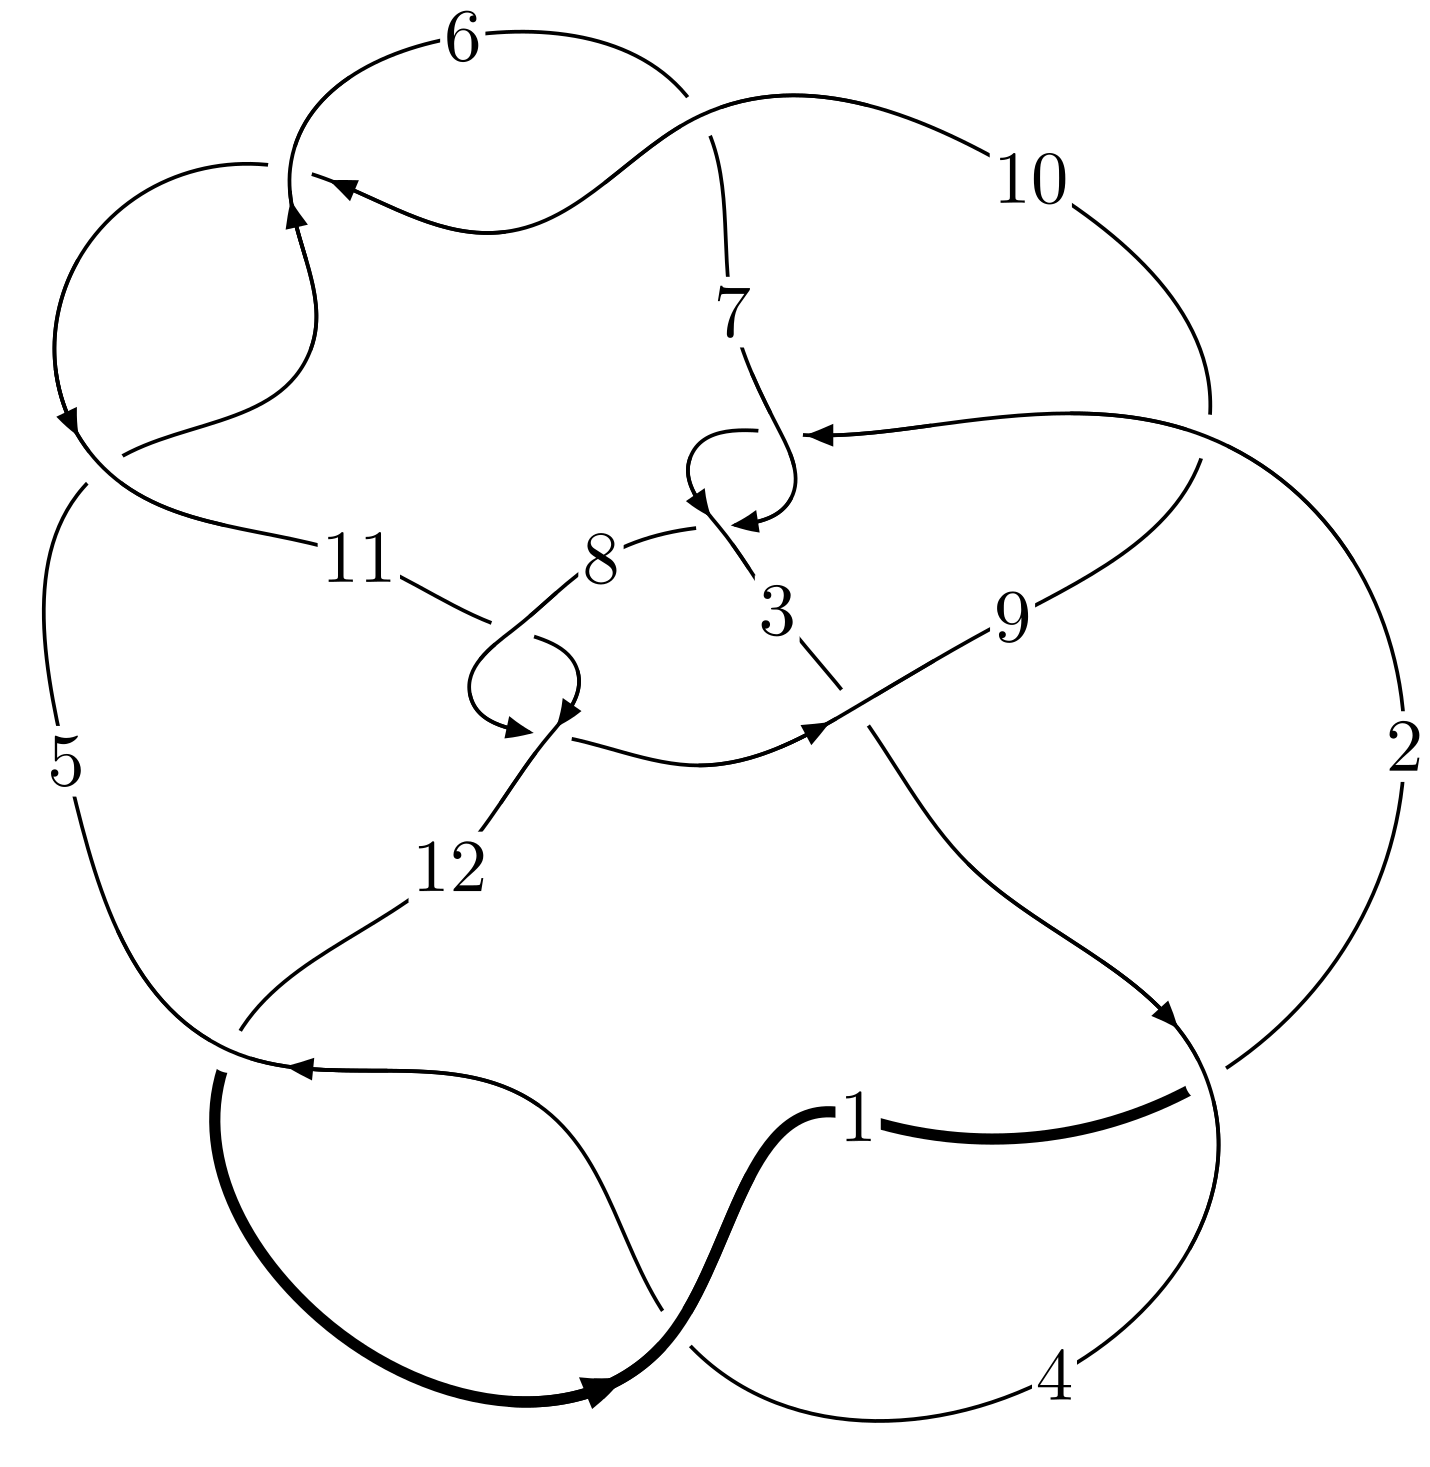
\includegraphics[width=112pt]{../../../GIT/diagram.site/Diagrams/png/1869_12a_1068.png}\\
\ \ \ A knot diagram\footnotemark}&
\allowdisplaybreaks
\textbf{Linearized knot diagam} \\
\cline{2-2}
 &
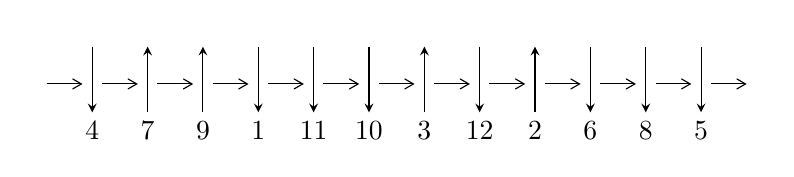
\begin{tikzpicture}[x=20pt, y=17pt]
	% nodes
	\node (C0) at (0, 0) {};
	\node (C1) at (1, 0) {};
	\node (C1U) at (1, +1) {};
	\node (C1D) at (1, -1) {4};

	\node (C2) at (2, 0) {};
	\node (C2U) at (2, +1) {};
	\node (C2D) at (2, -1) {7};

	\node (C3) at (3, 0) {};
	\node (C3U) at (3, +1) {};
	\node (C3D) at (3, -1) {9};

	\node (C4) at (4, 0) {};
	\node (C4U) at (4, +1) {};
	\node (C4D) at (4, -1) {1};

	\node (C5) at (5, 0) {};
	\node (C5U) at (5, +1) {};
	\node (C5D) at (5, -1) {11};

	\node (C6) at (6, 0) {};
	\node (C6U) at (6, +1) {};
	\node (C6D) at (6, -1) {10};

	\node (C7) at (7, 0) {};
	\node (C7U) at (7, +1) {};
	\node (C7D) at (7, -1) {3};

	\node (C8) at (8, 0) {};
	\node (C8U) at (8, +1) {};
	\node (C8D) at (8, -1) {12};

	\node (C9) at (9, 0) {};
	\node (C9U) at (9, +1) {};
	\node (C9D) at (9, -1) {2};

	\node (C10) at (10, 0) {};
	\node (C10U) at (10, +1) {};
	\node (C10D) at (10, -1) {6};

	\node (C11) at (11, 0) {};
	\node (C11U) at (11, +1) {};
	\node (C11D) at (11, -1) {8};

	\node (C12) at (12, 0) {};
	\node (C12U) at (12, +1) {};
	\node (C12D) at (12, -1) {5};
	\node (C13) at (13, 0) {};

	% arrows
	\draw[->,>={angle 60}]
	(C0) edge (C1) (C1) edge (C2) (C2) edge (C3) (C3) edge (C4) (C4) edge (C5) (C5) edge (C6) (C6) edge (C7) (C7) edge (C8) (C8) edge (C9) (C9) edge (C10) (C10) edge (C11) (C11) edge (C12) (C12) edge (C13) ;	\draw[->,>=stealth]
	(C1U) edge (C1D) (C2D) edge (C2U) (C3D) edge (C3U) (C4U) edge (C4D) (C5U) edge (C5D) (C6U) edge (C6D) (C7D) edge (C7U) (C8U) edge (C8D) (C9D) edge (C9U) (C10U) edge (C10D) (C11U) edge (C11D) (C12U) edge (C12D) ;
	\end{tikzpicture} \\
\hhline{~~} \\& 
\textbf{Solving Sequence} \\ \cline{2-2} 
 &
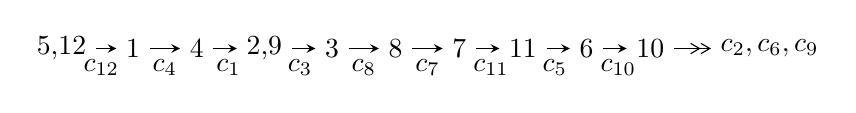
\begin{tikzpicture}[x=23pt, y=7pt]
	% node
	\node (A0) at (-1/8, 0) {5,12};
	\node (A1) at (1, 0) {1};
	\node (A2) at (2, 0) {4};
	\node (A3) at (49/16, 0) {2,9};
	\node (A4) at (33/8, 0) {3};
	\node (A5) at (41/8, 0) {8};
	\node (A6) at (49/8, 0) {7};
	\node (A7) at (57/8, 0) {11};
	\node (A8) at (65/8, 0) {6};
	\node (A9) at (73/8, 0) {10};
	\node (C1) at (1/2, -1) {$c_{12}$};
	\node (C2) at (3/2, -1) {$c_{4}$};
	\node (C3) at (5/2, -1) {$c_{1}$};
	\node (C4) at (29/8, -1) {$c_{3}$};
	\node (C5) at (37/8, -1) {$c_{8}$};
	\node (C6) at (45/8, -1) {$c_{7}$};
	\node (C7) at (53/8, -1) {$c_{11}$};
	\node (C8) at (61/8, -1) {$c_{5}$};
	\node (C9) at (69/8, -1) {$c_{10}$};
	\node (A10) at (11, 0) {$c_{2},c_{6},c_{9}$};

	% edge
	\draw[->,>=stealth]	
	(A0) edge (A1) (A1) edge (A2) (A2) edge (A3) (A3) edge (A4) (A4) edge (A5) (A5) edge (A6) (A6) edge (A7) (A7) edge (A8) (A8) edge (A9) ;
	\draw[->>,>={angle 60}]	
	(A9) edge (A10);
\end{tikzpicture} \\ 

\end{tabular} \\

\footnotetext{
The image of knot diagram is generated by the software ``\textbf{Draw programme}" developed by Andrew Bartholomew(\url{http://www.layer8.co.uk/maths/draw/index.htm\#Running-draw}), where we modified some parts for our purpose(\url{https://github.com/CATsTAILs/LinksPainter}).
}\phantom \\ \newline 
\centering \textbf{Ideals for irreducible components\footnotemark of $X_{\text{par}}$} 
 
\begin{align*}
I^u_{1}&=\langle 
1.50029\times10^{216} u^{98}+5.86036\times10^{216} u^{97}+\cdots+5.58008\times10^{215} b+1.44724\times10^{217},\\
\phantom{I^u_{1}}&\phantom{= \langle  }2.25470\times10^{216} u^{98}+9.19598\times10^{216} u^{97}+\cdots+5.58008\times10^{215} a+5.61430\times10^{217},\;u^{99}+4 u^{98}+\cdots+36 u+1\rangle \\
I^u_{2}&=\langle 
4 u^{26}-18 u^{25}+\cdots+b-3,\;-4 u^{26}+16 u^{25}+\cdots+a+4,\;u^{27}-3 u^{26}+\cdots-4 u+1\rangle \\
\\
\end{align*}
\raggedright * 2 irreducible components of $\dim_{\mathbb{C}}=0$, with total 126 representations.\\
\footnotetext{All coefficients of polynomials are rational numbers. But the coefficients are sometimes approximated in decimal forms when there is not enough margin.}
\newpage
\renewcommand{\arraystretch}{1}
\centering \section*{I. $I^u_{1}= \langle 1.50\times10^{216} u^{98}+5.86\times10^{216} u^{97}+\cdots+5.58\times10^{215} b+1.45\times10^{217},\;2.25\times10^{216} u^{98}+9.20\times10^{216} u^{97}+\cdots+5.58\times10^{215} a+5.61\times10^{217},\;u^{99}+4 u^{98}+\cdots+36 u+1 \rangle$}
\flushleft \textbf{(i) Arc colorings}\\
\begin{tabular}{m{7pt} m{180pt} m{7pt} m{180pt} }
\flushright $a_{5}=$&$\begin{pmatrix}0\\u\end{pmatrix}$ \\
\flushright $a_{12}=$&$\begin{pmatrix}1\\0\end{pmatrix}$ \\
\flushright $a_{1}=$&$\begin{pmatrix}1\\u^2\end{pmatrix}$ \\
\flushright $a_{4}=$&$\begin{pmatrix}u\\u^3+u\end{pmatrix}$ \\
\flushright $a_{2}=$&$\begin{pmatrix}u^2+1\\u^4+2 u^2\end{pmatrix}$ \\
\flushright $a_{9}=$&$\begin{pmatrix}-4.04062 u^{98}-16.4800 u^{97}+\cdots-2163.01 u-100.613\\-2.68866 u^{98}-10.5023 u^{97}+\cdots-730.857 u-25.9358\end{pmatrix}$ \\
\flushright $a_{3}=$&$\begin{pmatrix}29.0429 u^{98}+111.972 u^{97}+\cdots+6025.60 u+197.226\\-3.10791 u^{98}-12.2548 u^{97}+\cdots-840.423 u-33.7257\end{pmatrix}$ \\
\flushright $a_{8}=$&$\begin{pmatrix}-6.72927 u^{98}-26.9823 u^{97}+\cdots-2893.86 u-126.549\\-2.68866 u^{98}-10.5023 u^{97}+\cdots-730.857 u-25.9358\end{pmatrix}$ \\
\flushright $a_{7}=$&$\begin{pmatrix}-33.9952 u^{98}-132.268 u^{97}+\cdots-7939.55 u-282.211\\1.29259 u^{98}+4.98101 u^{97}+\cdots+349.365 u+15.2746\end{pmatrix}$ \\
\flushright $a_{11}=$&$\begin{pmatrix}41.3416 u^{98}+161.620 u^{97}+\cdots+11365.0 u+448.455\\3.78798 u^{98}+14.6203 u^{97}+\cdots+1051.78 u+38.9844\end{pmatrix}$ \\
\flushright $a_{6}=$&$\begin{pmatrix}17.7191 u^{98}+68.5869 u^{97}+\cdots+3201.82 u+77.1568\\-4.02761 u^{98}-15.3718 u^{97}+\cdots-1226.90 u-53.2891\end{pmatrix}$ \\
\flushright $a_{10}=$&$\begin{pmatrix}-7.06679 u^{98}-28.2694 u^{97}+\cdots-2947.05 u-127.980\\-2.76743 u^{98}-10.7591 u^{97}+\cdots-748.335 u-26.6011\end{pmatrix}$\\&\end{tabular}
\flushleft \textbf{(ii) Obstruction class $= -1$}\\~\\
\flushleft \textbf{(iii) Cusp Shapes $= 23.2492 u^{98}+90.4225 u^{97}+\cdots+5217.51 u+181.119$}\\~\\
\newpage\renewcommand{\arraystretch}{1}
\flushleft \textbf{(iv) u-Polynomials at the component}\newline \\
\begin{tabular}{m{50pt}|m{274pt}}
Crossings & \hspace{64pt}u-Polynomials at each crossing \\
\hline $$\begin{aligned}c_{1},c_{4},c_{12}\end{aligned}$$&$\begin{aligned}
&u^{99}-4 u^{98}+\cdots+36 u-1
\end{aligned}$\\
\hline $$\begin{aligned}c_{2},c_{7}\end{aligned}$$&$\begin{aligned}
&u^{99}+u^{98}+\cdots-2230 u-532
\end{aligned}$\\
\hline $$\begin{aligned}c_{3}\end{aligned}$$&$\begin{aligned}
&u^{99}- u^{98}+\cdots-127450 u+3749
\end{aligned}$\\
\hline $$\begin{aligned}c_{5},c_{6},c_{10}\end{aligned}$$&$\begin{aligned}
&u^{99}+u^{98}+\cdots+472 u-103
\end{aligned}$\\
\hline $$\begin{aligned}c_{8},c_{11}\end{aligned}$$&$\begin{aligned}
&u^{99}-24 u^{97}+\cdots-37 u+1
\end{aligned}$\\
\hline $$\begin{aligned}c_{9}\end{aligned}$$&$\begin{aligned}
&u^{99}+3 u^{98}+\cdots-3184124 u+9109661
\end{aligned}$\\
\hline
\end{tabular}\\~\\
\newpage\renewcommand{\arraystretch}{1}
\flushleft \textbf{(v) Riley Polynomials at the component}\newline \\
\begin{tabular}{m{50pt}|m{274pt}}
Crossings & \hspace{64pt}Riley Polynomials at each crossing \\
\hline $$\begin{aligned}c_{1},c_{4},c_{12}\end{aligned}$$&$\begin{aligned}
&y^{99}+104 y^{98}+\cdots+292 y-1
\end{aligned}$\\
\hline $$\begin{aligned}c_{2},c_{7}\end{aligned}$$&$\begin{aligned}
&y^{99}-73 y^{98}+\cdots+11428188 y-283024
\end{aligned}$\\
\hline $$\begin{aligned}c_{3}\end{aligned}$$&$\begin{aligned}
&y^{99}-27 y^{98}+\cdots+15140464222 y-14055001
\end{aligned}$\\
\hline $$\begin{aligned}c_{5},c_{6},c_{10}\end{aligned}$$&$\begin{aligned}
&y^{99}+109 y^{98}+\cdots-84774 y-10609
\end{aligned}$\\
\hline $$\begin{aligned}c_{8},c_{11}\end{aligned}$$&$\begin{aligned}
&y^{99}-48 y^{98}+\cdots+671 y-1
\end{aligned}$\\
\hline $$\begin{aligned}c_{9}\end{aligned}$$&$\begin{aligned}
&y^{99}-57 y^{98}+\cdots+2009455767939712 y-82985923534921
\end{aligned}$\\
\hline
\end{tabular}\\~\\
\newpage\flushleft \textbf{(vi) Complex Volumes and Cusp Shapes}
$$\begin{array}{c|c|c}  
\text{Solutions to }I^u_{1}& \I (\text{vol} + \sqrt{-1}CS) & \text{Cusp shape}\\
 \hline 
\begin{aligned}
u &= \phantom{-}0.380785 + 0.967960 I \\
a &= -1.078150 + 0.090070 I \\
b &= \phantom{-}0.999599 - 0.621542 I\end{aligned}
 & \phantom{-}7.29844 - 0.30926 I & \phantom{-0.000000 } 0 \\ \hline\begin{aligned}
u &= \phantom{-}0.380785 - 0.967960 I \\
a &= -1.078150 - 0.090070 I \\
b &= \phantom{-}0.999599 + 0.621542 I\end{aligned}
 & \phantom{-}7.29844 + 0.30926 I & \phantom{-0.000000 } 0 \\ \hline\begin{aligned}
u &= -0.916031 + 0.535204 I \\
a &= -0.575578 - 0.742046 I \\
b &= -1.138750 + 0.708186 I\end{aligned}
 & \phantom{-}8.2842 + 12.1910 I & \phantom{-0.000000 } 0 \\ \hline\begin{aligned}
u &= -0.916031 - 0.535204 I \\
a &= -0.575578 + 0.742046 I \\
b &= -1.138750 - 0.708186 I\end{aligned}
 & \phantom{-}8.2842 - 12.1910 I & \phantom{-0.000000 } 0 \\ \hline\begin{aligned}
u &= \phantom{-}0.081133 + 0.917673 I \\
a &= -0.891072 + 0.177720 I \\
b &= \phantom{-}0.291147 + 0.429752 I\end{aligned}
 & \phantom{-}4.97123 - 1.60465 I & \phantom{-0.000000 } 0 \\ \hline\begin{aligned}
u &= \phantom{-}0.081133 - 0.917673 I \\
a &= -0.891072 - 0.177720 I \\
b &= \phantom{-}0.291147 - 0.429752 I\end{aligned}
 & \phantom{-}4.97123 + 1.60465 I & \phantom{-0.000000 } 0 \\ \hline\begin{aligned}
u &= -0.861368 + 0.321070 I \\
a &= -1.299810 - 0.217264 I \\
b &= -0.810628 + 0.586401 I\end{aligned}
 & \phantom{-}9.09344 - 1.46018 I & \phantom{-0.000000 } 0 \\ \hline\begin{aligned}
u &= -0.861368 - 0.321070 I \\
a &= -1.299810 + 0.217264 I \\
b &= -0.810628 - 0.586401 I\end{aligned}
 & \phantom{-}9.09344 + 1.46018 I & \phantom{-0.000000 } 0 \\ \hline\begin{aligned}
u &= \phantom{-}0.190324 + 1.068550 I \\
a &= -0.237611 + 0.115075 I \\
b &= -1.257530 - 0.134290 I\end{aligned}
 & \phantom{-}0.28001 - 2.62311 I & \phantom{-0.000000 } 0 \\ \hline\begin{aligned}
u &= \phantom{-}0.190324 - 1.068550 I \\
a &= -0.237611 - 0.115075 I \\
b &= -1.257530 + 0.134290 I\end{aligned}
 & \phantom{-}0.28001 + 2.62311 I & \phantom{-0.000000 } 0\\
 \hline 
 \end{array}$$\newpage$$\begin{array}{c|c|c}  
\text{Solutions to }I^u_{1}& \I (\text{vol} + \sqrt{-1}CS) & \text{Cusp shape}\\
 \hline 
\begin{aligned}
u &= \phantom{-}0.808953 + 0.423145 I \\
a &= \phantom{-}0.554722 - 0.715807 I \\
b &= \phantom{-}0.989338 + 0.318623 I\end{aligned}
 & -2.61211 - 3.25013 I & \phantom{-0.000000 } 0 \\ \hline\begin{aligned}
u &= \phantom{-}0.808953 - 0.423145 I \\
a &= \phantom{-}0.554722 + 0.715807 I \\
b &= \phantom{-}0.989338 - 0.318623 I\end{aligned}
 & -2.61211 + 3.25013 I & \phantom{-0.000000 } 0 \\ \hline\begin{aligned}
u &= \phantom{-}0.634538 + 0.901713 I \\
a &= \phantom{-}0.140566 - 0.301929 I \\
b &= \phantom{-}0.868536 - 0.046181 I\end{aligned}
 & -1.32841 - 1.88863 I & \phantom{-0.000000 } 0 \\ \hline\begin{aligned}
u &= \phantom{-}0.634538 - 0.901713 I \\
a &= \phantom{-}0.140566 + 0.301929 I \\
b &= \phantom{-}0.868536 + 0.046181 I\end{aligned}
 & -1.32841 + 1.88863 I & \phantom{-0.000000 } 0 \\ \hline\begin{aligned}
u &= \phantom{-}0.994467 + 0.486650 I \\
a &= -0.691397 + 0.442067 I \\
b &= -1.033900 - 0.585558 I\end{aligned}
 & \phantom{-}3.54877 - 5.37076 I & \phantom{-0.000000 } 0 \\ \hline\begin{aligned}
u &= \phantom{-}0.994467 - 0.486650 I \\
a &= -0.691397 - 0.442067 I \\
b &= -1.033900 + 0.585558 I\end{aligned}
 & \phantom{-}3.54877 + 5.37076 I & \phantom{-0.000000 } 0 \\ \hline\begin{aligned}
u &= -0.715566 + 0.532179 I \\
a &= \phantom{-}0.457943 + 1.155560 I \\
b &= \phantom{-}1.145500 - 0.504808 I\end{aligned}
 & \phantom{-}0.80367 + 8.22347 I & \phantom{-0.000000 } 0 \\ \hline\begin{aligned}
u &= -0.715566 - 0.532179 I \\
a &= \phantom{-}0.457943 - 1.155560 I \\
b &= \phantom{-}1.145500 + 0.504808 I\end{aligned}
 & \phantom{-}0.80367 - 8.22347 I & \phantom{-0.000000 } 0 \\ \hline\begin{aligned}
u &= -0.574131 + 0.616338 I \\
a &= -0.268689 + 0.221406 I \\
b &= -0.447700 - 0.999113 I\end{aligned}
 & \phantom{-}10.34210 + 6.07405 I & \phantom{-0.000000 } 0 \\ \hline\begin{aligned}
u &= -0.574131 - 0.616338 I \\
a &= -0.268689 - 0.221406 I \\
b &= -0.447700 + 0.999113 I\end{aligned}
 & \phantom{-}10.34210 - 6.07405 I & \phantom{-0.000000 } 0\\
 \hline 
 \end{array}$$\newpage$$\begin{array}{c|c|c}  
\text{Solutions to }I^u_{1}& \I (\text{vol} + \sqrt{-1}CS) & \text{Cusp shape}\\
 \hline 
\begin{aligned}
u &= -0.907557 + 0.730013 I \\
a &= \phantom{-}0.124855 - 0.182401 I \\
b &= -0.906542 - 0.595760 I\end{aligned}
 & \phantom{-}8.77349 - 6.14037 I & \phantom{-0.000000 } 0 \\ \hline\begin{aligned}
u &= -0.907557 - 0.730013 I \\
a &= \phantom{-}0.124855 + 0.182401 I \\
b &= -0.906542 + 0.595760 I\end{aligned}
 & \phantom{-}8.77349 + 6.14037 I & \phantom{-0.000000 } 0 \\ \hline\begin{aligned}
u &= -0.622216 + 0.510793 I \\
a &= -0.042605 + 0.326293 I \\
b &= \phantom{-}1.068350 + 0.348839 I\end{aligned}
 & \phantom{-}0.80525 - 3.61642 I & \phantom{-0.000000 } 0 \\ \hline\begin{aligned}
u &= -0.622216 - 0.510793 I \\
a &= -0.042605 - 0.326293 I \\
b &= \phantom{-}1.068350 - 0.348839 I\end{aligned}
 & \phantom{-}0.80525 + 3.61642 I & \phantom{-0.000000 } 0 \\ \hline\begin{aligned}
u &= \phantom{-}0.770064 + 0.954381 I \\
a &= -0.082133 + 0.202671 I \\
b &= -0.628584 + 0.505927 I\end{aligned}
 & \phantom{-}4.90385 - 0.82779 I & \phantom{-0.000000 } 0 \\ \hline\begin{aligned}
u &= \phantom{-}0.770064 - 0.954381 I \\
a &= -0.082133 - 0.202671 I \\
b &= -0.628584 - 0.505927 I\end{aligned}
 & \phantom{-}4.90385 + 0.82779 I & \phantom{-0.000000 } 0 \\ \hline\begin{aligned}
u &= -0.123577 + 1.234730 I \\
a &= -1.06774 - 1.68429 I \\
b &= \phantom{-}0.0518778 - 0.0095839 I\end{aligned}
 & \phantom{-}10.91520 + 4.80273 I & \phantom{-0.000000 } 0 \\ \hline\begin{aligned}
u &= -0.123577 - 1.234730 I \\
a &= -1.06774 + 1.68429 I \\
b &= \phantom{-}0.0518778 + 0.0095839 I\end{aligned}
 & \phantom{-}10.91520 - 4.80273 I & \phantom{-0.000000 } 0 \\ \hline\begin{aligned}
u &= -0.003388 + 1.272120 I \\
a &= \phantom{-}0.915951 - 0.583969 I \\
b &= -1.52579 + 0.30597 I\end{aligned}
 & \phantom{-}1.48489 + 1.58514 I & \phantom{-0.000000 } 0 \\ \hline\begin{aligned}
u &= -0.003388 - 1.272120 I \\
a &= \phantom{-}0.915951 + 0.583969 I \\
b &= -1.52579 - 0.30597 I\end{aligned}
 & \phantom{-}1.48489 - 1.58514 I & \phantom{-0.000000 } 0\\
 \hline 
 \end{array}$$\newpage$$\begin{array}{c|c|c}  
\text{Solutions to }I^u_{1}& \I (\text{vol} + \sqrt{-1}CS) & \text{Cusp shape}\\
 \hline 
\begin{aligned}
u &= -0.240720 + 1.252590 I \\
a &= -1.038950 + 0.271205 I \\
b &= \phantom{-}1.124750 + 0.115853 I\end{aligned}
 & \phantom{-}6.14932 - 1.00815 I & \phantom{-0.000000 } 0 \\ \hline\begin{aligned}
u &= -0.240720 - 1.252590 I \\
a &= -1.038950 - 0.271205 I \\
b &= \phantom{-}1.124750 - 0.115853 I\end{aligned}
 & \phantom{-}6.14932 + 1.00815 I & \phantom{-0.000000 } 0 \\ \hline\begin{aligned}
u &= \phantom{-}0.709928 + 0.123175 I \\
a &= \phantom{-}0.663884 - 0.511483 I \\
b &= \phantom{-}1.052080 + 0.916210 I\end{aligned}
 & \phantom{-}4.65542 - 3.59845 I & \phantom{-0.000000 } 0 \\ \hline\begin{aligned}
u &= \phantom{-}0.709928 - 0.123175 I \\
a &= \phantom{-}0.663884 + 0.511483 I \\
b &= \phantom{-}1.052080 - 0.916210 I\end{aligned}
 & \phantom{-}4.65542 + 3.59845 I & \phantom{-0.000000 } 0 \\ \hline\begin{aligned}
u &= -0.372442 + 0.611930 I \\
a &= \phantom{-}0.58103 - 1.74962 I \\
b &= -1.095300 + 0.309250 I\end{aligned}
 & \phantom{-}0.26345 + 2.62023 I & \phantom{-0.000000 } 0 \\ \hline\begin{aligned}
u &= -0.372442 - 0.611930 I \\
a &= \phantom{-}0.58103 + 1.74962 I \\
b &= -1.095300 - 0.309250 I\end{aligned}
 & \phantom{-}0.26345 - 2.62023 I & \phantom{-0.000000 } 0 \\ \hline\begin{aligned}
u &= \phantom{-}0.584980 + 0.353698 I \\
a &= -0.030160 + 1.413860 I \\
b &= -0.894830 - 0.022267 I\end{aligned}
 & -1.45461 - 0.14764 I & \phantom{-0.000000 } 0 \\ \hline\begin{aligned}
u &= \phantom{-}0.584980 - 0.353698 I \\
a &= -0.030160 - 1.413860 I \\
b &= -0.894830 + 0.022267 I\end{aligned}
 & -1.45461 + 0.14764 I & \phantom{-0.000000 } 0 \\ \hline\begin{aligned}
u &= \phantom{-}0.236471 + 1.318320 I \\
a &= -0.05193 - 2.23086 I \\
b &= \phantom{-}0.93339 + 1.19290 I\end{aligned}
 & \phantom{-}9.12685 - 6.97856 I & \phantom{-0.000000 } 0 \\ \hline\begin{aligned}
u &= \phantom{-}0.236471 - 1.318320 I \\
a &= -0.05193 + 2.23086 I \\
b &= \phantom{-}0.93339 - 1.19290 I\end{aligned}
 & \phantom{-}9.12685 + 6.97856 I & \phantom{-0.000000 } 0\\
 \hline 
 \end{array}$$\newpage$$\begin{array}{c|c|c}  
\text{Solutions to }I^u_{1}& \I (\text{vol} + \sqrt{-1}CS) & \text{Cusp shape}\\
 \hline 
\begin{aligned}
u &= -0.484489 + 0.446016 I \\
a &= -0.222432 - 0.700483 I \\
b &= \phantom{-}0.180754 + 0.863249 I\end{aligned}
 & \phantom{-}3.72537 + 3.36221 I & \phantom{-0.000000 } 0 \\ \hline\begin{aligned}
u &= -0.484489 - 0.446016 I \\
a &= -0.222432 + 0.700483 I \\
b &= \phantom{-}0.180754 - 0.863249 I\end{aligned}
 & \phantom{-}3.72537 - 3.36221 I & \phantom{-0.000000 } 0 \\ \hline\begin{aligned}
u &= -0.071334 + 1.372250 I \\
a &= \phantom{-}0.48461 - 1.50093 I \\
b &= -1.028430 + 0.639743 I\end{aligned}
 & \phantom{-}2.79128 + 1.44895 I & \phantom{-0.000000 } 0 \\ \hline\begin{aligned}
u &= -0.071334 - 1.372250 I \\
a &= \phantom{-}0.48461 + 1.50093 I \\
b &= -1.028430 - 0.639743 I\end{aligned}
 & \phantom{-}2.79128 - 1.44895 I & \phantom{-0.000000 } 0 \\ \hline\begin{aligned}
u &= -0.145077 + 1.385060 I \\
a &= -0.27987 + 1.86042 I \\
b &= \phantom{-}1.18889 - 0.99715 I\end{aligned}
 & \phantom{-}7.12843 + 5.25158 I & \phantom{-0.000000 } 0 \\ \hline\begin{aligned}
u &= -0.145077 - 1.385060 I \\
a &= -0.27987 - 1.86042 I \\
b &= \phantom{-}1.18889 + 0.99715 I\end{aligned}
 & \phantom{-}7.12843 - 5.25158 I & \phantom{-0.000000 } 0 \\ \hline\begin{aligned}
u &= \phantom{-}0.086189 + 1.400630 I \\
a &= -0.351019 + 1.124700 I \\
b &= \phantom{-}0.475218 - 0.574761 I\end{aligned}
 & \phantom{-}5.31989 - 2.36934 I & \phantom{-0.000000 } 0 \\ \hline\begin{aligned}
u &= \phantom{-}0.086189 - 1.400630 I \\
a &= -0.351019 - 1.124700 I \\
b &= \phantom{-}0.475218 + 0.574761 I\end{aligned}
 & \phantom{-}5.31989 + 2.36934 I & \phantom{-0.000000 } 0 \\ \hline\begin{aligned}
u &= \phantom{-}0.152955 + 1.396230 I \\
a &= \phantom{-}0.54193 + 1.75034 I \\
b &= -0.931903 - 0.988146 I\end{aligned}
 & \phantom{-}4.04235 - 4.91926 I & \phantom{-0.000000 } 0 \\ \hline\begin{aligned}
u &= \phantom{-}0.152955 - 1.396230 I \\
a &= \phantom{-}0.54193 - 1.75034 I \\
b &= -0.931903 + 0.988146 I\end{aligned}
 & \phantom{-}4.04235 + 4.91926 I & \phantom{-0.000000 } 0\\
 \hline 
 \end{array}$$\newpage$$\begin{array}{c|c|c}  
\text{Solutions to }I^u_{1}& \I (\text{vol} + \sqrt{-1}CS) & \text{Cusp shape}\\
 \hline 
\begin{aligned}
u &= -0.547574 + 0.214398 I \\
a &= \phantom{-}1.56284 + 0.57855 I \\
b &= \phantom{-}0.239576 - 0.404718 I\end{aligned}
 & \phantom{-}3.17897 - 0.15464 I & \phantom{-}2.53527 - 1.97824 I \\ \hline\begin{aligned}
u &= -0.547574 - 0.214398 I \\
a &= \phantom{-}1.56284 - 0.57855 I \\
b &= \phantom{-}0.239576 + 0.404718 I\end{aligned}
 & \phantom{-}3.17897 + 0.15464 I & \phantom{-}2.53527 + 1.97824 I \\ \hline\begin{aligned}
u &= -0.02049 + 1.42222 I \\
a &= -0.701489 + 0.531251 I \\
b &= \phantom{-}1.79195 - 0.31139 I\end{aligned}
 & \phantom{-}6.70624 + 2.98104 I & \phantom{-0.000000 } 0 \\ \hline\begin{aligned}
u &= -0.02049 - 1.42222 I \\
a &= -0.701489 - 0.531251 I \\
b &= \phantom{-}1.79195 + 0.31139 I\end{aligned}
 & \phantom{-}6.70624 - 2.98104 I & \phantom{-0.000000 } 0 \\ \hline\begin{aligned}
u &= -0.27716 + 1.40128 I \\
a &= \phantom{-}0.45484 + 1.34405 I \\
b &= \phantom{-}0.712181 - 0.569531 I\end{aligned}
 & \phantom{-}8.25008 + 3.15430 I & \phantom{-0.000000 } 0 \\ \hline\begin{aligned}
u &= -0.27716 - 1.40128 I \\
a &= \phantom{-}0.45484 - 1.34405 I \\
b &= \phantom{-}0.712181 + 0.569531 I\end{aligned}
 & \phantom{-}8.25008 - 3.15430 I & \phantom{-0.000000 } 0 \\ \hline\begin{aligned}
u &= -0.01731 + 1.43658 I \\
a &= \phantom{-}0.16463 + 1.87472 I \\
b &= -0.790510 - 0.509312 I\end{aligned}
 & \phantom{-}8.08050 + 0.40274 I & \phantom{-0.000000 } 0 \\ \hline\begin{aligned}
u &= -0.01731 - 1.43658 I \\
a &= \phantom{-}0.16463 - 1.87472 I \\
b &= -0.790510 + 0.509312 I\end{aligned}
 & \phantom{-}8.08050 - 0.40274 I & \phantom{-0.000000 } 0 \\ \hline\begin{aligned}
u &= -0.00477 + 1.46661 I \\
a &= -0.862324 - 1.050040 I \\
b &= \phantom{-}0.947756 + 0.787724 I\end{aligned}
 & \phantom{-}7.01175 - 2.09262 I & \phantom{-0.000000 } 0 \\ \hline\begin{aligned}
u &= -0.00477 - 1.46661 I \\
a &= -0.862324 + 1.050040 I \\
b &= \phantom{-}0.947756 - 0.787724 I\end{aligned}
 & \phantom{-}7.01175 + 2.09262 I & \phantom{-0.000000 } 0\\
 \hline 
 \end{array}$$\newpage$$\begin{array}{c|c|c}  
\text{Solutions to }I^u_{1}& \I (\text{vol} + \sqrt{-1}CS) & \text{Cusp shape}\\
 \hline 
\begin{aligned}
u &= -0.15332 + 1.46090 I \\
a &= -0.55488 - 1.56502 I \\
b &= \phantom{-}0.389356 + 1.027810 I\end{aligned}
 & \phantom{-}9.89339 + 5.67837 I & \phantom{-0.000000 } 0 \\ \hline\begin{aligned}
u &= -0.15332 - 1.46090 I \\
a &= -0.55488 + 1.56502 I \\
b &= \phantom{-}0.389356 - 1.027810 I\end{aligned}
 & \phantom{-}9.89339 - 5.67837 I & \phantom{-0.000000 } 0 \\ \hline\begin{aligned}
u &= \phantom{-}0.450858 + 0.256702 I \\
a &= -0.177543 + 0.990337 I \\
b &= -1.071810 - 0.572179 I\end{aligned}
 & -1.22302 - 2.67007 I & -7.39915 + 10.94039 I \\ \hline\begin{aligned}
u &= \phantom{-}0.450858 - 0.256702 I \\
a &= -0.177543 - 0.990337 I \\
b &= -1.071810 + 0.572179 I\end{aligned}
 & -1.22302 + 2.67007 I & -7.39915 - 10.94039 I \\ \hline\begin{aligned}
u &= \phantom{-}0.22256 + 1.46568 I \\
a &= \phantom{-}0.390336 + 1.238280 I \\
b &= -0.623858 - 0.415482 I\end{aligned}
 & \phantom{-}4.50771 - 3.11816 I & \phantom{-0.000000 } 0 \\ \hline\begin{aligned}
u &= \phantom{-}0.22256 - 1.46568 I \\
a &= \phantom{-}0.390336 - 1.238280 I \\
b &= -0.623858 + 0.415482 I\end{aligned}
 & \phantom{-}4.50771 + 3.11816 I & \phantom{-0.000000 } 0 \\ \hline\begin{aligned}
u &= \phantom{-}0.06659 + 1.48445 I \\
a &= \phantom{-}0.271142 - 1.371170 I \\
b &= \phantom{-}1.164310 + 0.524284 I\end{aligned}
 & \phantom{-}14.4517 - 5.4304 I & \phantom{-0.000000 } 0 \\ \hline\begin{aligned}
u &= \phantom{-}0.06659 - 1.48445 I \\
a &= \phantom{-}0.271142 + 1.371170 I \\
b &= \phantom{-}1.164310 - 0.524284 I\end{aligned}
 & \phantom{-}14.4517 + 5.4304 I & \phantom{-0.000000 } 0 \\ \hline\begin{aligned}
u &= -0.488613\phantom{ +0.000000I} \\
a &= -0.894239\phantom{ +0.000000I} \\
b &= -1.17090\phantom{ +0.000000I}\end{aligned}
 & -1.64387\phantom{ +0.000000I} & -8.18420\phantom{ +0.000000I} \\ \hline\begin{aligned}
u &= \phantom{-}0.27861 + 1.49474 I \\
a &= -0.22098 - 1.40771 I \\
b &= \phantom{-}1.061660 + 0.599311 I\end{aligned}
 & \phantom{-}3.61668 - 7.15621 I & \phantom{-0.000000 } 0\\
 \hline 
 \end{array}$$\newpage$$\begin{array}{c|c|c}  
\text{Solutions to }I^u_{1}& \I (\text{vol} + \sqrt{-1}CS) & \text{Cusp shape}\\
 \hline 
\begin{aligned}
u &= \phantom{-}0.27861 - 1.49474 I \\
a &= -0.22098 + 1.40771 I \\
b &= \phantom{-}1.061660 - 0.599311 I\end{aligned}
 & \phantom{-}3.61668 + 7.15621 I & \phantom{-0.000000 } 0 \\ \hline\begin{aligned}
u &= -0.446853 + 0.111335 I \\
a &= \phantom{-}1.50560 - 0.11020 I \\
b &= \phantom{-}1.052330 - 0.677785 I\end{aligned}
 & \phantom{-}2.28317 + 3.15343 I & \phantom{-}4.58442 + 1.03106 I \\ \hline\begin{aligned}
u &= -0.446853 - 0.111335 I \\
a &= \phantom{-}1.50560 + 0.11020 I \\
b &= \phantom{-}1.052330 + 0.677785 I\end{aligned}
 & \phantom{-}2.28317 - 3.15343 I & \phantom{-}4.58442 - 1.03106 I \\ \hline\begin{aligned}
u &= -0.19941 + 1.53402 I \\
a &= \phantom{-}0.61915 + 1.37411 I \\
b &= -0.60331 - 1.38982 I\end{aligned}
 & \phantom{-}17.3600 + 8.9631 I & \phantom{-0.000000 } 0 \\ \hline\begin{aligned}
u &= -0.19941 - 1.53402 I \\
a &= \phantom{-}0.61915 - 1.37411 I \\
b &= -0.60331 + 1.38982 I\end{aligned}
 & \phantom{-}17.3600 - 8.9631 I & \phantom{-0.000000 } 0 \\ \hline\begin{aligned}
u &= -0.36021 + 1.51331 I \\
a &= -0.258402 - 1.132070 I \\
b &= -1.158180 + 0.594833 I\end{aligned}
 & \phantom{-}15.0187 + 3.1095 I & \phantom{-0.000000 } 0 \\ \hline\begin{aligned}
u &= -0.36021 - 1.51331 I \\
a &= -0.258402 + 1.132070 I \\
b &= -1.158180 - 0.594833 I\end{aligned}
 & \phantom{-}15.0187 - 3.1095 I & \phantom{-0.000000 } 0 \\ \hline\begin{aligned}
u &= -0.24901 + 1.53942 I \\
a &= -0.40345 + 1.63875 I \\
b &= \phantom{-}1.158500 - 0.694088 I\end{aligned}
 & \phantom{-}7.60750 + 11.78010 I & \phantom{-0.000000 } 0 \\ \hline\begin{aligned}
u &= -0.24901 - 1.53942 I \\
a &= -0.40345 - 1.63875 I \\
b &= \phantom{-}1.158500 + 0.694088 I\end{aligned}
 & \phantom{-}7.60750 - 11.78010 I & \phantom{-0.000000 } 0 \\ \hline\begin{aligned}
u &= -0.14537 + 1.56497 I \\
a &= \phantom{-}0.82793 - 1.44795 I \\
b &= -0.931355 + 0.541931 I\end{aligned}
 & \phantom{-}7.58537 + 4.66034 I & \phantom{-0.000000 } 0\\
 \hline 
 \end{array}$$\newpage$$\begin{array}{c|c|c}  
\text{Solutions to }I^u_{1}& \I (\text{vol} + \sqrt{-1}CS) & \text{Cusp shape}\\
 \hline 
\begin{aligned}
u &= -0.14537 - 1.56497 I \\
a &= \phantom{-}0.82793 + 1.44795 I \\
b &= -0.931355 - 0.541931 I\end{aligned}
 & \phantom{-}7.58537 - 4.66034 I & \phantom{-0.000000 } 0 \\ \hline\begin{aligned}
u &= \phantom{-}0.303921 + 0.301418 I \\
a &= \phantom{-}0.484939 + 0.687513 I \\
b &= -0.050441 - 0.295647 I\end{aligned}
 & -0.151501 - 0.860358 I & -3.67340 + 7.82157 I \\ \hline\begin{aligned}
u &= \phantom{-}0.303921 - 0.301418 I \\
a &= \phantom{-}0.484939 - 0.687513 I \\
b &= -0.050441 + 0.295647 I\end{aligned}
 & -0.151501 + 0.860358 I & -3.67340 - 7.82157 I \\ \hline\begin{aligned}
u &= \phantom{-}0.14950 + 1.57868 I \\
a &= \phantom{-}0.218886 - 1.212920 I \\
b &= -0.266157 + 1.215160 I\end{aligned}
 & \phantom{-}13.34460 - 3.44425 I & \phantom{-0.000000 } 0 \\ \hline\begin{aligned}
u &= \phantom{-}0.14950 - 1.57868 I \\
a &= \phantom{-}0.218886 + 1.212920 I \\
b &= -0.266157 - 1.215160 I\end{aligned}
 & \phantom{-}13.34460 + 3.44425 I & \phantom{-0.000000 } 0 \\ \hline\begin{aligned}
u &= -0.32728 + 1.55643 I \\
a &= \phantom{-}0.17280 - 1.59481 I \\
b &= -1.27617 + 0.85627 I\end{aligned}
 & \phantom{-}15.0673 + 16.7358 I & \phantom{-0.000000 } 0 \\ \hline\begin{aligned}
u &= -0.32728 - 1.55643 I \\
a &= \phantom{-}0.17280 + 1.59481 I \\
b &= -1.27617 - 0.85627 I\end{aligned}
 & \phantom{-}15.0673 - 16.7358 I & \phantom{-0.000000 } 0 \\ \hline\begin{aligned}
u &= \phantom{-}0.34061 + 1.56064 I \\
a &= \phantom{-}0.104948 + 1.330500 I \\
b &= -1.28754 - 0.72555 I\end{aligned}
 & \phantom{-}10.2362 - 10.1957 I & \phantom{-0.000000 } 0 \\ \hline\begin{aligned}
u &= \phantom{-}0.34061 - 1.56064 I \\
a &= \phantom{-}0.104948 - 1.330500 I \\
b &= -1.28754 + 0.72555 I\end{aligned}
 & \phantom{-}10.2362 + 10.1957 I & \phantom{-0.000000 } 0 \\ \hline\begin{aligned}
u &= -0.391447\phantom{ +0.000000I} \\
a &= -1.50474\phantom{ +0.000000I} \\
b &= -1.03773\phantom{ +0.000000I}\end{aligned}
 & -1.66971\phantom{ +0.000000I} & -6.70640\phantom{ +0.000000I}\\
 \hline 
 \end{array}$$\newpage$$\begin{array}{c|c|c}  
\text{Solutions to }I^u_{1}& \I (\text{vol} + \sqrt{-1}CS) & \text{Cusp shape}\\
 \hline 
\begin{aligned}
u &= \phantom{-}0.132488 + 0.329921 I \\
a &= \phantom{-}4.62802 - 2.84343 I \\
b &= \phantom{-}0.770323 + 0.470588 I\end{aligned}
 & \phantom{-}8.28620 - 4.57392 I & \phantom{-}2.18985 + 8.66184 I \\ \hline\begin{aligned}
u &= \phantom{-}0.132488 - 0.329921 I \\
a &= \phantom{-}4.62802 + 2.84343 I \\
b &= \phantom{-}0.770323 - 0.470588 I\end{aligned}
 & \phantom{-}8.28620 + 4.57392 I & \phantom{-}2.18985 - 8.66184 I \\ \hline\begin{aligned}
u &= -0.00439 + 1.69977 I \\
a &= -0.715193 + 0.460101 I \\
b &= \phantom{-}0.467243 - 0.410517 I\end{aligned}
 & \phantom{-}16.8314 - 1.2465 I & \phantom{-0.000000 } 0 \\ \hline\begin{aligned}
u &= -0.00439 - 1.69977 I \\
a &= -0.715193 - 0.460101 I \\
b &= \phantom{-}0.467243 + 0.410517 I\end{aligned}
 & \phantom{-}16.8314 + 1.2465 I & \phantom{-0.000000 } 0 \\ \hline\begin{aligned}
u &= -0.19462 + 1.71124 I \\
a &= \phantom{-}0.288108 + 0.497754 I \\
b &= -0.442079 - 0.604819 I\end{aligned}
 & \phantom{-}17.2396 - 1.7990 I & \phantom{-0.000000 } 0 \\ \hline\begin{aligned}
u &= -0.19462 - 1.71124 I \\
a &= \phantom{-}0.288108 - 0.497754 I \\
b &= -0.442079 + 0.604819 I\end{aligned}
 & \phantom{-}17.2396 + 1.7990 I & \phantom{-0.000000 } 0 \\ \hline\begin{aligned}
u &= -0.125192\phantom{ +0.000000I} \\
a &= \phantom{-}13.2053\phantom{ +0.000000I} \\
b &= -0.469237\phantom{ +0.000000I}\end{aligned}
 & \phantom{-}2.89635\phantom{ +0.000000I} & \phantom{-}10.3080\phantom{ +0.000000I} \\ \hline\begin{aligned}
u &= -0.0876198 + 0.0177221 I \\
a &= \phantom{-}4.04055 - 8.18611 I \\
b &= \phantom{-}1.41561 - 0.34626 I\end{aligned}
 & \phantom{-}1.67204 + 2.65205 I & -6.65996 + 0.50003 I \\ \hline\begin{aligned}
u &= -0.0876198 - 0.0177221 I \\
a &= \phantom{-}4.04055 + 8.18611 I \\
b &= \phantom{-}1.41561 + 0.34626 I\end{aligned}
 & \phantom{-}1.67204 - 2.65205 I & -6.65996 - 0.50003 I\\
 \hline 
 \end{array}$$\newpage\newpage\renewcommand{\arraystretch}{1}
\centering \section*{II. $I^u_{2}= \langle 4 u^{26}-18 u^{25}+\cdots+b-3,\;-4 u^{26}+16 u^{25}+\cdots+a+4,\;u^{27}-3 u^{26}+\cdots-4 u+1 \rangle$}
\flushleft \textbf{(i) Arc colorings}\\
\begin{tabular}{m{7pt} m{180pt} m{7pt} m{180pt} }
\flushright $a_{5}=$&$\begin{pmatrix}0\\u\end{pmatrix}$ \\
\flushright $a_{12}=$&$\begin{pmatrix}1\\0\end{pmatrix}$ \\
\flushright $a_{1}=$&$\begin{pmatrix}1\\u^2\end{pmatrix}$ \\
\flushright $a_{4}=$&$\begin{pmatrix}u\\u^3+u\end{pmatrix}$ \\
\flushright $a_{2}=$&$\begin{pmatrix}u^2+1\\u^4+2 u^2\end{pmatrix}$ \\
\flushright $a_{9}=$&$\begin{pmatrix}4 u^{26}-16 u^{25}+\cdots+24 u-4\\-4 u^{26}+18 u^{25}+\cdots-20 u+3\end{pmatrix}$ \\
\flushright $a_{3}=$&$\begin{pmatrix}-3 u^{26}+9 u^{25}+\cdots-10 u+4\\u^{24}-3 u^{23}+\cdots+7 u-2\end{pmatrix}$ \\
\flushright $a_{8}=$&$\begin{pmatrix}2 u^{25}-6 u^{24}+\cdots+4 u-1\\-4 u^{26}+18 u^{25}+\cdots-20 u+3\end{pmatrix}$ \\
\flushright $a_{7}=$&$\begin{pmatrix}u^4- u^3+3 u^2-2 u+2\\3 u^{26}- u^{25}+\cdots-9 u+2\end{pmatrix}$ \\
\flushright $a_{11}=$&$\begin{pmatrix}u^{26}+2 u^{25}+\cdots-3 u+2\\2 u^{26}-6 u^{25}+\cdots-9 u^2-1\end{pmatrix}$ \\
\flushright $a_{6}=$&$\begin{pmatrix}- u^{26}+3 u^{25}+\cdots-5 u^2+2 u\\10 u^{26}-20 u^{25}+\cdots-8 u+3\end{pmatrix}$ \\
\flushright $a_{10}=$&$\begin{pmatrix}- u^{25}+3 u^{24}+\cdots+8 u-1\\-6 u^{26}+30 u^{25}+\cdots-39 u+8\end{pmatrix}$\\&\end{tabular}
\flushleft \textbf{(ii) Obstruction class $= 1$}\\~\\
\flushleft \textbf{(iii) Cusp Shapes $= -7 u^{26}-6 u^{25}-57 u^{24}-163 u^{23}+27 u^{22}-1594 u^{21}+2054 u^{20}-8129 u^{19}+10974 u^{18}-24708 u^{17}+29721 u^{16}-47186 u^{15}+47876 u^{14}-57143 u^{13}+47152 u^{12}-42833 u^{11}+27674 u^{10}-18847 u^9+9241 u^8-4614 u^7+1745 u^6-573 u^5+22 u^4+118 u^3-150 u^2+57 u-22$}\\~\\
\newpage\renewcommand{\arraystretch}{1}
\flushleft \textbf{(iv) u-Polynomials at the component}\newline \\
\begin{tabular}{m{50pt}|m{274pt}}
Crossings & \hspace{64pt}u-Polynomials at each crossing \\
\hline $$\begin{aligned}c_{1},c_{12}\end{aligned}$$&$\begin{aligned}
&u^{27}-3 u^{26}+\cdots-4 u+1
\end{aligned}$\\
\hline $$\begin{aligned}c_{2}\end{aligned}$$&$\begin{aligned}
&u^{27}-9 u^{25}+\cdots-7 u^2+1
\end{aligned}$\\
\hline $$\begin{aligned}c_{3}\end{aligned}$$&$\begin{aligned}
&u^{27}-2 u^{24}+\cdots+11 u^2+1
\end{aligned}$\\
\hline $$\begin{aligned}c_{4}\end{aligned}$$&$\begin{aligned}
&u^{27}+3 u^{26}+\cdots-4 u-1
\end{aligned}$\\
\hline $$\begin{aligned}c_{5},c_{6}\end{aligned}$$&$\begin{aligned}
&u^{27}+16 u^{25}+\cdots-6 u+1
\end{aligned}$\\
\hline $$\begin{aligned}c_{7}\end{aligned}$$&$\begin{aligned}
&u^{27}-9 u^{25}+\cdots+7 u^2-1
\end{aligned}$\\
\hline $$\begin{aligned}c_{8}\end{aligned}$$&$\begin{aligned}
&u^{27}+5 u^{26}+\cdots-5 u-1
\end{aligned}$\\
\hline $$\begin{aligned}c_{9}\end{aligned}$$&$\begin{aligned}
&u^{27}-5 u^{25}+\cdots-6 u+1
\end{aligned}$\\
\hline $$\begin{aligned}c_{10}\end{aligned}$$&$\begin{aligned}
&u^{27}+16 u^{25}+\cdots-6 u-1
\end{aligned}$\\
\hline $$\begin{aligned}c_{11}\end{aligned}$$&$\begin{aligned}
&u^{27}-5 u^{26}+\cdots-5 u+1
\end{aligned}$\\
\hline
\end{tabular}\\~\\
\newpage\renewcommand{\arraystretch}{1}
\flushleft \textbf{(v) Riley Polynomials at the component}\newline \\
\begin{tabular}{m{50pt}|m{274pt}}
Crossings & \hspace{64pt}Riley Polynomials at each crossing \\
\hline $$\begin{aligned}c_{1},c_{4},c_{12}\end{aligned}$$&$\begin{aligned}
&y^{27}+31 y^{26}+\cdots-8 y-1
\end{aligned}$\\
\hline $$\begin{aligned}c_{2},c_{7}\end{aligned}$$&$\begin{aligned}
&y^{27}-18 y^{26}+\cdots+14 y-1
\end{aligned}$\\
\hline $$\begin{aligned}c_{3}\end{aligned}$$&$\begin{aligned}
&y^{27}-14 y^{25}+\cdots-22 y-1
\end{aligned}$\\
\hline $$\begin{aligned}c_{5},c_{6},c_{10}\end{aligned}$$&$\begin{aligned}
&y^{27}+32 y^{26}+\cdots-6 y-1
\end{aligned}$\\
\hline $$\begin{aligned}c_{8},c_{11}\end{aligned}$$&$\begin{aligned}
&y^{27}-21 y^{26}+\cdots+27 y-1
\end{aligned}$\\
\hline $$\begin{aligned}c_{9}\end{aligned}$$&$\begin{aligned}
&y^{27}-10 y^{26}+\cdots-32 y-1
\end{aligned}$\\
\hline
\end{tabular}\\~\\
\newpage\flushleft \textbf{(vi) Complex Volumes and Cusp Shapes}
$$\begin{array}{c|c|c}  
\text{Solutions to }I^u_{2}& \I (\text{vol} + \sqrt{-1}CS) & \text{Cusp shape}\\
 \hline 
\begin{aligned}
u &= \phantom{-}0.529825 + 0.809918 I \\
a &= -0.055011 + 0.489943 I \\
b &= -0.957191 - 0.078245 I\end{aligned}
 & -1.56306 - 2.18322 I & -8.36006 + 8.63349 I \\ \hline\begin{aligned}
u &= \phantom{-}0.529825 - 0.809918 I \\
a &= -0.055011 - 0.489943 I \\
b &= -0.957191 + 0.078245 I\end{aligned}
 & -1.56306 + 2.18322 I & -8.36006 - 8.63349 I \\ \hline\begin{aligned}
u &= \phantom{-}0.267042 + 0.760078 I \\
a &= \phantom{-}0.751964 - 0.351572 I \\
b &= \phantom{-}1.266910 + 0.279218 I\end{aligned}
 & \phantom{-}2.31208 - 3.21416 I & \phantom{-}1.95146 + 4.84868 I \\ \hline\begin{aligned}
u &= \phantom{-}0.267042 - 0.760078 I \\
a &= \phantom{-}0.751964 + 0.351572 I \\
b &= \phantom{-}1.266910 - 0.279218 I\end{aligned}
 & \phantom{-}2.31208 + 3.21416 I & \phantom{-}1.95146 - 4.84868 I \\ \hline\begin{aligned}
u &= \phantom{-}0.567361 + 1.110970 I \\
a &= -0.431431 - 0.330212 I \\
b &= \phantom{-}0.774453 - 0.350896 I\end{aligned}
 & \phantom{-}4.00066 - 0.48119 I & -3.66135 - 1.00155 I \\ \hline\begin{aligned}
u &= \phantom{-}0.567361 - 1.110970 I \\
a &= -0.431431 + 0.330212 I \\
b &= \phantom{-}0.774453 + 0.350896 I\end{aligned}
 & \phantom{-}4.00066 + 0.48119 I & -3.66135 + 1.00155 I \\ \hline\begin{aligned}
u &= \phantom{-}0.059850 + 1.252320 I \\
a &= -1.65356 + 0.39903 I \\
b &= \phantom{-}1.67176 - 0.45128 I\end{aligned}
 & \phantom{-}4.67985 + 2.02941 I & -2.20493 - 2.90597 I \\ \hline\begin{aligned}
u &= \phantom{-}0.059850 - 1.252320 I \\
a &= -1.65356 - 0.39903 I \\
b &= \phantom{-}1.67176 + 0.45128 I\end{aligned}
 & \phantom{-}4.67985 - 2.02941 I & -2.20493 + 2.90597 I \\ \hline\begin{aligned}
u &= -0.174494 + 1.271190 I \\
a &= \phantom{-}0.90134 + 2.08409 I \\
b &= \phantom{-}0.721752 - 0.620445 I\end{aligned}
 & \phantom{-}11.02560 + 5.82117 I & \phantom{-}4.75059 - 7.23956 I \\ \hline\begin{aligned}
u &= -0.174494 - 1.271190 I \\
a &= \phantom{-}0.90134 - 2.08409 I \\
b &= \phantom{-}0.721752 + 0.620445 I\end{aligned}
 & \phantom{-}11.02560 - 5.82117 I & \phantom{-}4.75059 + 7.23956 I\\
 \hline 
 \end{array}$$\newpage$$\begin{array}{c|c|c}  
\text{Solutions to }I^u_{2}& \I (\text{vol} + \sqrt{-1}CS) & \text{Cusp shape}\\
 \hline 
\begin{aligned}
u &= \phantom{-}0.030883 + 1.290990 I \\
a &= \phantom{-}0.478980 - 0.478805 I \\
b &= -1.45287 + 0.32069 I\end{aligned}
 & \phantom{-}2.18015 + 1.34894 I & \phantom{-}4.75960 + 0. I\phantom{ +0.000000I} \\ \hline\begin{aligned}
u &= \phantom{-}0.030883 - 1.290990 I \\
a &= \phantom{-}0.478980 + 0.478805 I \\
b &= -1.45287 - 0.32069 I\end{aligned}
 & \phantom{-}2.18015 - 1.34894 I & \phantom{-}4.75960 + 0. I\phantom{ +0.000000I} \\ \hline\begin{aligned}
u &= -0.391975 + 0.461539 I \\
a &= \phantom{-}0.09757 + 2.50345 I \\
b &= \phantom{-}0.588105 + 0.363259 I\end{aligned}
 & \phantom{-}8.14039 - 3.78112 I & -0.034946 - 0.532297 I \\ \hline\begin{aligned}
u &= -0.391975 - 0.461539 I \\
a &= \phantom{-}0.09757 - 2.50345 I \\
b &= \phantom{-}0.588105 - 0.363259 I\end{aligned}
 & \phantom{-}8.14039 + 3.78112 I & -0.034946 + 0.532297 I \\ \hline\begin{aligned}
u &= \phantom{-}0.192166 + 1.399840 I \\
a &= -0.28477 - 1.97334 I \\
b &= \phantom{-}1.11005 + 1.12524 I\end{aligned}
 & \phantom{-}7.14619 - 6.16599 I & \phantom{-}1.37328 + 7.84994 I \\ \hline\begin{aligned}
u &= \phantom{-}0.192166 - 1.399840 I \\
a &= -0.28477 + 1.97334 I \\
b &= \phantom{-}1.11005 - 1.12524 I\end{aligned}
 & \phantom{-}7.14619 + 6.16599 I & \phantom{-}1.37328 - 7.84994 I \\ \hline\begin{aligned}
u &= \phantom{-}0.530911 + 0.240216 I \\
a &= \phantom{-}0.905097 - 0.380887 I \\
b &= \phantom{-}1.159280 + 0.725401 I\end{aligned}
 & \phantom{-}1.91060 - 3.56104 I & -5.75759 + 9.42146 I \\ \hline\begin{aligned}
u &= \phantom{-}0.530911 - 0.240216 I \\
a &= \phantom{-}0.905097 + 0.380887 I \\
b &= \phantom{-}1.159280 - 0.725401 I\end{aligned}
 & \phantom{-}1.91060 + 3.56104 I & -5.75759 - 9.42146 I \\ \hline\begin{aligned}
u &= -0.20013 + 1.42433 I \\
a &= -0.07006 - 1.51288 I \\
b &= -0.607531 + 0.291383 I\end{aligned}
 & \phantom{-}7.48897 + 2.36651 I & \phantom{-0.000000 }      -6
0. 10   - 0.822434 I \\ \hline\begin{aligned}
u &= -0.20013 - 1.42433 I \\
a &= -0.07006 + 1.51288 I \\
b &= -0.607531 - 0.291383 I\end{aligned}
 & \phantom{-}7.48897 - 2.36651 I & \phantom{-0.000000 -}     -6
0. 10   + 0.822434 I\\
 \hline 
 \end{array}$$\newpage$$\begin{array}{c|c|c}  
\text{Solutions to }I^u_{2}& \I (\text{vol} + \sqrt{-1}CS) & \text{Cusp shape}\\
 \hline 
\begin{aligned}
u &= \phantom{-}0.17269 + 1.48110 I \\
a &= \phantom{-}0.57866 + 1.32623 I \\
b &= -0.752363 - 0.679230 I\end{aligned}
 & \phantom{-}5.10932 - 3.84763 I & \phantom{-}3.16616 + 5.03771 I \\ \hline\begin{aligned}
u &= \phantom{-}0.17269 - 1.48110 I \\
a &= \phantom{-}0.57866 - 1.32623 I \\
b &= -0.752363 + 0.679230 I\end{aligned}
 & \phantom{-}5.10932 + 3.84763 I & \phantom{-}3.16616 - 5.03771 I \\ \hline\begin{aligned}
u &= -0.433229\phantom{ +0.000000I} \\
a &= -3.79438\phantom{ +0.000000I} \\
b &= -0.627919\phantom{ +0.000000I}\end{aligned}
 & \phantom{-}2.54905\phantom{ +0.000000I} & -14.0320\phantom{ +0.000000I} \\ \hline\begin{aligned}
u &= \phantom{-}0.215989 + 0.342402 I \\
a &= \phantom{-}1.17353 + 1.40885 I \\
b &= -1.110620 - 0.350103 I\end{aligned}
 & -1.11587 - 1.97397 I & -6.20655 + 0.29675 I \\ \hline\begin{aligned}
u &= \phantom{-}0.215989 - 0.342402 I \\
a &= \phantom{-}1.17353 - 1.40885 I \\
b &= -1.110620 + 0.350103 I\end{aligned}
 & -1.11587 + 1.97397 I & -6.20655 - 0.29675 I \\ \hline\begin{aligned}
u &= -0.08350 + 1.73493 I \\
a &= -0.495123 + 0.240156 I \\
b &= \phantom{-}0.402235 + 0.073150 I\end{aligned}
 & \phantom{-}16.4978 - 1.6817 I & \phantom{-0.000000 } 0 \\ \hline\begin{aligned}
u &= -0.08350 - 1.73493 I \\
a &= -0.495123 - 0.240156 I \\
b &= \phantom{-}0.402235 - 0.073150 I\end{aligned}
 & \phantom{-}16.4978 + 1.6817 I & \phantom{-0.000000 } 0\\
 \hline 
 \end{array}$$\newpage
\newpage\renewcommand{\arraystretch}{1}
\centering \section*{ III. u-Polynomials}
\begin{tabular}{m{50pt}|m{274pt}}
Crossings & \hspace{64pt}u-Polynomials at each crossing \\
\hline $$\begin{aligned}c_{1},c_{12}\end{aligned}$$&$\begin{aligned}
&(u^{27}-3 u^{26}+\cdots-4 u+1)(u^{99}-4 u^{98}+\cdots+36 u-1)
\end{aligned}$\\
\hline $$\begin{aligned}c_{2}\end{aligned}$$&$\begin{aligned}
&(u^{27}-9 u^{25}+\cdots-7 u^2+1)(u^{99}+u^{98}+\cdots-2230 u-532)
\end{aligned}$\\
\hline $$\begin{aligned}c_{3}\end{aligned}$$&$\begin{aligned}
&(u^{27}-2 u^{24}+\cdots+11 u^2+1)(u^{99}- u^{98}+\cdots-127450 u+3749)
\end{aligned}$\\
\hline $$\begin{aligned}c_{4}\end{aligned}$$&$\begin{aligned}
&(u^{27}+3 u^{26}+\cdots-4 u-1)(u^{99}-4 u^{98}+\cdots+36 u-1)
\end{aligned}$\\
\hline $$\begin{aligned}c_{5},c_{6}\end{aligned}$$&$\begin{aligned}
&(u^{27}+16 u^{25}+\cdots-6 u+1)(u^{99}+u^{98}+\cdots+472 u-103)
\end{aligned}$\\
\hline $$\begin{aligned}c_{7}\end{aligned}$$&$\begin{aligned}
&(u^{27}-9 u^{25}+\cdots+7 u^2-1)(u^{99}+u^{98}+\cdots-2230 u-532)
\end{aligned}$\\
\hline $$\begin{aligned}c_{8}\end{aligned}$$&$\begin{aligned}
&(u^{27}+5 u^{26}+\cdots-5 u-1)(u^{99}-24 u^{97}+\cdots-37 u+1)
\end{aligned}$\\
\hline $$\begin{aligned}c_{9}\end{aligned}$$&$\begin{aligned}
&(u^{27}-5 u^{25}+\cdots-6 u+1)(u^{99}+3 u^{98}+\cdots-3184124 u+9109661)
\end{aligned}$\\
\hline $$\begin{aligned}c_{10}\end{aligned}$$&$\begin{aligned}
&(u^{27}+16 u^{25}+\cdots-6 u-1)(u^{99}+u^{98}+\cdots+472 u-103)
\end{aligned}$\\
\hline $$\begin{aligned}c_{11}\end{aligned}$$&$\begin{aligned}
&(u^{27}-5 u^{26}+\cdots-5 u+1)(u^{99}-24 u^{97}+\cdots-37 u+1)
\end{aligned}$\\
\hline
\end{tabular}\newpage\renewcommand{\arraystretch}{1}
\centering \section*{ IV. Riley Polynomials}
\begin{tabular}{m{50pt}|m{274pt}}
Crossings & \hspace{64pt}Riley Polynomials at each crossing \\
\hline $$\begin{aligned}c_{1},c_{4},c_{12}\end{aligned}$$&$\begin{aligned}
&(y^{27}+31 y^{26}+\cdots-8 y-1)(y^{99}+104 y^{98}+\cdots+292 y-1)
\end{aligned}$\\
\hline $$\begin{aligned}c_{2},c_{7}\end{aligned}$$&$\begin{aligned}
&(y^{27}-18 y^{26}+\cdots+14 y-1)\\
&\cdot(y^{99}-73 y^{98}+\cdots+11428188 y-283024)
\end{aligned}$\\
\hline $$\begin{aligned}c_{3}\end{aligned}$$&$\begin{aligned}
&(y^{27}-14 y^{25}+\cdots-22 y-1)\\
&\cdot(y^{99}-27 y^{98}+\cdots+15140464222 y-14055001)
\end{aligned}$\\
\hline $$\begin{aligned}c_{5},c_{6},c_{10}\end{aligned}$$&$\begin{aligned}
&(y^{27}+32 y^{26}+\cdots-6 y-1)(y^{99}+109 y^{98}+\cdots-84774 y-10609)
\end{aligned}$\\
\hline $$\begin{aligned}c_{8},c_{11}\end{aligned}$$&$\begin{aligned}
&(y^{27}-21 y^{26}+\cdots+27 y-1)(y^{99}-48 y^{98}+\cdots+671 y-1)
\end{aligned}$\\
\hline $$\begin{aligned}c_{9}\end{aligned}$$&$\begin{aligned}
&(y^{27}-10 y^{26}+\cdots-32 y-1)\\
&\cdot(y^{99}-57 y^{98}+\cdots+2009455767939712 y-82985923534921)
\end{aligned}$\\
\hline
\end{tabular}
\vskip 2pc
\end{document}